\chapter{Advanced attacks against SGX Enclaves}
\label{chp:advanced-threats} 

%The solutions in~\ref{chp:static-protection} 
%and~\ref{chp:runtime-protection-untrusted} enhance static and runtime 
%protection of untrusted code in memory, respectively.
%What happens when the attacker focuses on the TEE itself?
%
%The answer to this question is addressed in the paper:
%\begin{itemize}
%	\item SnakeGX: a sneaky attack against SGX Enclaves (ACNS 2021).
%\end{itemize}
%
%The strong isolation introduced by  stimulated researchers and practitioners 
%to develop new attacks 
%vectors~\cite{foreshadow,Murdock2019plundervolt,203183,lee2017hacking}.
%Among them, an interesting research line is to exploit memory-corruption 
%errors 
%inside the enclave code and run one-shot code-reuse 
%attacks to steal enclave secrets (\eg cryptographic 
%keys)~\cite{geometry2007}.
%Recently, we observed many solutions that identify such flaws in 
%enclaves~\cite{teerex,tale-two-worlds} and new code-reuse techniques 
%tailored for SGX~\cite{lee2017hacking,biondo2018guard}.
%First, Lee et al. discussed Dark-ROP~\cite{lee2017hacking}
%that combines a colluded OS and oracles to identify gadgets for 
%return-oriented programming (ROP)~\cite{geometry2007}.
%An advanced technique was proposed by Biondo et al. with Guard's 
%Dilemma~\cite{biondo2018guard} that does not require the assistance of the OS 
%to perform the attack.
%%The main limitation of this attack is the need of crashing the victim
%%enclave many times in order to craft the actual payload.
%%To cope with this issue, Biondo et at. proposed Guard's 
%%Dilemma~\cite{biondo2018guard} that uses particular gadgets already present 
%%in 
%%the Intel Software 
%%Development Kit (SDK) to build the payload without any enclave crashes.
%%Moreover, Dilemma requires only an unprivileged attacker to carry out a 
%%single 
%%one-shot attack and steal secrets from an enclave.

In this chapter, we explore a new attack scenario a in which an adversary 
attempts at taking control of a TEE \emph{enclave} while hiding its presence 
from the operating system.
%In this scenario, however, the authors did not consider an OS that may employ 
%existing memory forensic techniques to identify the 
%intrusions~\cite{stancill2013check,polychronakis2011rop,kittel2015counteracting,Graziano:2016:RFA:2897845.2897894}.
%For instance, in case of external intrusion into a remote server running SGX 
%enclaves, the adversary is also interested in reducing the amount 
%of traces left; otherwise, analysts may detect the intrusion and act 
%consequently.
%This is even more critical in case the enclave secret changes and the 
%adversary has to repeat the attack many times.
More precisely, we pose the following new research question:

\emph{Can we carry out an attack against SGX enclaves without being 
	noticed by an healthy Operating System?}

%We answer this doubt with an analysis of actual memory-forensic techniques
%to detect code-reuse attacks in memory.
%Our observations show that an analyst can use current memory-forensic 
%techniques to detect code-reuse payloads outside the enclave 
%(Section~\ref{sec:background}).
%Unfortunately, it comes as no surprise one can also abuse the security
%and privacy guarantees SGX offers; a recent line of research sees
%enclaves as secure containers to conceal malicious
%code~\cite{amsterdamsgxmalwer,schwarz2017malware,sgx-rop}. Albeit
%successful, such research require the attacker to obtain a legitimate
%license from Intel~\cite{intel-license} to integrate the malicious
%code in the enclave---a strong assumption that limits the realistic
%deployment of such threats.
We answer this question with a new approach that pushes further the 
stealthiness of code-reuse attacks in non-compromised OSs.
Our intuition is to implant a permanent payload inside the target 
enclave as a backdoor, thus exploiting the SGX protections to avoid 
inspection.
%
Our strategy definitely overcomes the limitations of the state-of-the-art;
the adversary does not need to repeat the attack and we minimize the 
traces left.
%
We implement our intuition in SnakeGX, a framework to implant
data-only backdoors in legitimate enclaves. 
We build on the concept of data-only
malware~\cite{vogl2014persistent} but extend it with a novel
architecture to adhere to the strict requirements of SGX environments.

%Cosa proponi?
%Un attacco che è persistent, stateful e interactive
Contrary to prior one-shot attacks~\cite{biondo2018guard,lee2017hacking}, our 
backdoor acts as an additional secure function (Section~\ref{sec:enclavekit}), 
which is: 
\begin{enumerate*}[label=(\roman*)]
	\item \textbf{persistent} in the context of the enclave,
	\item \textbf{stateful} as it maintains an internal state,
	\item \textbf{interactive} with the host by means of seamless context 
	switches.
\end{enumerate*}
%Come hai fatto?
%E' persistent perchè hai usato XYZ, è stateful perchè hai usato ABC, etc
Core to this is the identification of a design flaw that
affects the Intel SGX Software Development Kit (SDK) and allows an attacker to 
trigger arbitrary code in enclaves 
(Section~\ref{sec:sgx-internal})\footnote{We reported the flawed 
	behavior to Intel, which acknowledged it.}.
%which we abuse to implant a data-only backdoor.
%Come bypassi lo stato dell'arte?
%comprometti un enclave senza variarne il comportamento; non vieni identificato 
%da un OS; etc etc 
SnakeGX facilitates the creation of versatile backdoors concealed in
enclaves that evade memory forensic analysis by inheriting all the benefits SGX 
provides.
%We do not see our work as a mere academic exercise nor as a one-way offensive 
%research.
%On the contrary, 
Our aim is to raise awareness of TEEs---and SGX in particular---and how 
attackers may abuse that, which requires the community to reason more on the 
need of monitoring systems and advanced forensic techniques for SGX.

We evaluate the properties of SnakeGX against StealthDB~\cite{stealthdb}, an
open-source project that implements an encrypted database on top of SGX 
enclaves.
In particular, StealthDB uses dynamically generated AES keys to protect the
database's fields, thus urging the need of multiple one-shot attacks.
SnakeGX exfiltrates the keys upon the verification of specific conditions 
with a minimum footprint.
Our evaluation focuses on three aspects of SnakeGX 
(Section~\ref{sec:evaluation_snakegx}).
First, we illustrate our use-case: we show how SnakeGX achieves its goals
while preserving the original functionality of the enclave.
Second, we measure and compare the stealthiness of SnakeGX against the 
state-of-the-art.
Finally, we discuss possible countermeasures.
%Our technique requires a modest amount of 56 bytes to activate arbitrary long 
%and complex attacks while removing the burning of crafting new payloads.
%\todo{how and why do I measure the stealthiness of my attack in terms of 
%memory allocated? Give an hint}
%SnakeGX facilitates the creation of our attack, which requires a
%modest amount of 56 bytes to activate arbitrary long and complex
%payloads.
%In addition, SnakeGX's persistency, statefulness, and interactiveness
%properties preserve the original functionality of the enclave
%(Section~\ref{sec:evaluation_snakegx}).

In summary, we make the following contributions:
\begin{itemize}
	\item We propose SnakeGX, a framework built around an Intel SGX 
	SDK design flaw (Section~\ref{sec:sgx-internal}), and a novel architecture
	designed to create persistent, stateful, and interactive data-only
	malware for SGX (Section~\ref{sec:enclavekit}).
	\item We demonstrate the feasibility of SnakeGX on a real-world
	open source project\footnote{SnakeGX's source code is available 
		at~\url{https://github.com/tregua87/snakegx}.}.
	\item We measure and compare the attack footprint with current SGX 
	state-of-the-art techniques (Section~\ref{sec:evaluation_snakegx}).
\end{itemize}


\section{Threat Model and Assumptions}
\label{sec:threat-model_snakegx}

In this section, we first describe our threat model.
Then, we perform a preliminary analysis to measure the widespread of our 
assumptions over real SGX open-source projects.

\paragraph{\textbf{Threat Model.}}
One of the differences between SnakeGX and the previous one-shot code-reuse 
works is in the threat model.
Advanced code-reuse techniques require an unprivileged 
attacker~\cite{biondo2018guard}.
However, a non-compromised host can identify the presence of an adversary
in the system memory (Section~\ref{ssec:code-reuse-sgx}).
Therefore, we have to consider three players in our scenarios: the attacker, 
the victim enclave, and the host.
%Since we focus on code-reuse attacks, we rule out other techniques such as 
%micro-architectural or side-channel ones.
Below, we list their requirements, respectively.

%The payload can pursue different goals such as exfiltrating private 
%information 
%(\eg password saved in the enclave) or altering the behaviour of the secure 
%functions (\eg tampering with crypto keys in an enclave).
%Its activation, instead, leaves a minimal and less intrusive footprint.

\textbf{Attacker Capabilities.}
In our scenario, the attacker is highly motivated and has the following 
assumptions:

\begin{itemize}
	\item \textbf{The enclave contains a memory corruption vulnerability.}  
	The adversary is aware of a memory corruption error (\eg a buffer overflow) 
	in the target enclave.
	This error can be exploited to take control of the enclave itself.
	Having a memory-corruption is an assumption already taken by similar 
	works~\cite{biondo2018guard,lee2017hacking}.
	This is even more likely in projects that use SGX as a sub-system 
	container~\cite{baumann2015shielding,203255,seo2017sgx,199364}.
	Such projects host out-of-the-box software and, therefore, enclaves inherit 
	their vulnerabilities.
	\item \textbf{A code-reuse technique.} 
	SnakeGX does not require any specific code-reuse techniques (\eg ROP, 
	JOP, BROP, SROP) as long as this enables the attacker to take control of 
	the enclave execution. For the sake of simplicity, we use 
	the term \emph{chain} to indicate a generic code-reuse payload 
	(\eg a ROP-chain).
	\item \textbf{Knowledge of victim enclave memory layout.} 
	The attacker can infer the memory layout by inspecting the victim 
	address-space.
	It is also possible to leak memory information from within the enclave, as
	also assumed in~\cite{biondo2018guard}.
	\item \textbf{Adversary Location.} In our scenario, the adversary 
	resides in user-space. SnakeGX will reduce the adversary
	footprint, thus evading standard memory forensic 	
	techniques~\cite{stancill2013check,polychronakis2011rop,kittel2015counteracting,Graziano:2016:RFA:2897845.2897894},
	whose effectiveness relies on the amount of traces left in memory 
	(see Section~\ref{ssec:code-reuse-sgx}).
	%	\item \textbf{(Temporary) Host process control.}
	%	The attacker needs a partial control of the victim process for a short 
	%	period of time.
	%	More precisely, the attacker may need to inspect \texttt{uRts} to find 
	%and 
	%disable a trusted thread at installation phase.
	%	Since SGX allows reading the untrusted memory, this operation can be 
	%	performed from within the enclave.
	%	Moreover, the payload may interact with the host OS to exfiltrate data 
	%(\ie 
	%through a socket).
	%	Therefore, SnakeGX can potentially leave the enclave for a short amount 
	%of time.
	%	Modern malware-enclave works describe reliable techniques to achieve 
	%host-process control from within an enclave~\cite{sgx-rop}.
\end{itemize}

\textbf{Enclaves Capabilities.}
These are the assumptions for the enclave:

\begin{itemize}
	\item \textbf{Legitimate enclaves.} 
	The system contains one or more running enclaves.
	It is possible to exploit enclaves based on both SGX $1.0$ or $2.0$.
	\item \textbf{Intel SGX SDK usage.} 
	The victim enclave should be implemented by using the standard Intel SGX 
	Software Development Kit (SDK), we tested our approach with all the SDK 
	versions currently available.\footnote{At the time of writing, the last SDK 
		version is $2.9$.}
	This is a reasonable assumption since the Intel SGX SDK provides a 
	framework for developing applications on different OSs: Linux and Windows.
	\item \textbf{Multi-threading.}
	%	This is not strictly required, but for a more general approach would be 
	%ideal that the victim enclave has at least two threads.
	This is not strictly required, but the victim enclave should have
	at least two threads for a more general approach.
	The rationale behind this requirement is that the proposed implementation 
	may disable a trusted thread~\cite{intel-developer-guide} and in case of a 
	single-thread application this is a problem.  
	An enclave without free threads cannot 
	process secure functions, thus attracting the analysts attention.
	We might partially ease this requirement with the introduction of SGX 
	$2.0$. 
	% that allows the generation of new enclave pages at run-time.
	%	Another viable approach is to exploit some enclave misconfigurations, 
	%as 
	%explained in Section~\ref{ssec:memory-location}, 
	%	but this is a less generic solution.
	However, multi-thread enclaves are a reasonable assumption since different 
	open-source projects 
	use already this feature~\cite{sqlite-sgx,sgxtor,signal,203255,stealthdb} 
	and SGX-based applications are growing in complexity.
\end{itemize}

\textbf{Host Capabilities.}
This is the assumption for the host:

\begin{itemize}
	\item \textbf{Memory Inspection.}  The host can inspect the 
	processes memory and use standard approaches to detect traces of previous
	or ongoing 
	attacks~\cite{stancill2013check,polychronakis2011rop,kittel2015counteracting,Graziano:2016:RFA:2897845.2897894}.
\end{itemize}

We extend the threat model of previous works~\cite{biondo2018guard} 
by assuming the host can perform memory forensic analysis.
Therefore, an adversary has the need of hiding her presence in the machine 
and minimizing the interactions with the victim enclave.

\paragraph{\textbf{Preliminary Analysis of Assumptions.}}
%We collected a set of $27$ stand-alone SGX open-source projects from an online 
%hub~\cite{asop} to investigate the correctness of our assumptions and shown 
%in  
%Table~\ref{tbl:sgx-open-source-prj}.
%The results show that among the $27$ projects, $24$ of them were based on the 
%Intel SGX SDK, while others were developed with Graphene~\cite{203255}, Open 
%Enclave SDK~\cite{openenclave}, or contained mocked enclaves.
%From the Intel SGX SDK based projects, we counted $31$ enclaves in total, 
%among which $24$ were multi-threading ($77\%$).
%This preliminary analysis indicates that our threat model fulfills 
%real scenarios.
% OLD
We collected a set of $27$ stand-alone SGX open-source projects from an online 
hub~\cite{asop} to investigate the correctness of our assumptions (see full 
list in Appendix~\ref{app:preliminary-analysis-assumptions}).
The results show that among the $27$ projects, $24$ of them were based on the 
Intel SGX SDK, while others were developed with Graphene~\cite{203255}, Open 
Enclave SDK~\cite{openenclave}, or contained mocked enclaves.
From the Intel SGX SDK based projects, we counted $31$ enclaves in total, 
among which $24$ were multi-threading ($77\%$).
This preliminary analysis indicates that our threat model fulfills 
real scenarios.
Furthermore, we discuss the porting of SnakeGX over SDKs other than the Intel 
one in Section~\ref{sec:discussion_snakegx}.

\section{Intel SGX SDK Design Limitation}
%\section{SGX Enclaves Custom Trigger}
\label{sec:sgx-internal}
%\todo{highlight the importance of this part. This is crucial because the 
%consequence of thsi trick is havin a reliable hook that also reduces to zero 
%(almost) the effort of an attacker to attack an enclave repetitely.}

%A fundamental feature of SnakeGX is the ability of implanting new secure 
%functions in an enclave without altering its behavior.
%SnakeGX achieves this goal through a design error that affects all 
%the SGX Software Development Kit (SDK) versions released by Intel.

SnakeGX can trigger a payload inside the enclave without the need of repeating 
a new attack.
This feature is challenging because the enclave has a fixed 
entry point, thus an adversary cannot activate arbitrary code inside the 
enclave from the untrusted memory.
SnakeGX achieves this goal through a design error that affects all 
the SGX Software Development Kit (SDK) versions released by Intel.
In this section, we make a deep analysis of the Intel SGX SDK in order to 
highlight these issues and propose possible mitigations.

\subsection{SDK Overview}
\label{ssec:sdk-overview}

SGX specifications define only basic primitives for creating and interacting 
with an enclave.
Thus, Intel also provides an SDK that helps building SGX-based applications.
The Intel SGX SDK contains a run-time library that is composed by two parts: an 
untrusted run-time library (\texttt{uRts}) that is contained in the host 
process, and a trusted run-time library (\texttt{tRts}) that is contained in 
the enclave.
Specifically, \texttt{uRts} handles operations like multi-threading, while 
\texttt{tRts} manages secure functions dispatching and context-switch. 

The Intel SGX SDK exposes a set of APIs that are built on top of the leaf 
functions described in Section~\ref{sec:background}.
\texttt{ECALL}, \texttt{ERET}, \texttt{OCALL}, and \texttt{ORET} are the most 
important APIs for SnakeGX.
Figure~\ref{fig:synch-exit} shows the interaction between the host process and 
the enclave.
At the beginning, the host process invokes a secure function by using an 
\texttt{ECALL}, which is implemented by means of an \texttt{EENTER} 
(Figure~\ref{fig:synch-exit}, step $1$).
%At this point, the execution starts from the \texttt{OENTRY} address, which is 
%indicated by the input TCS (see Section~\ref{ssec:enclave-intreaction}).
%\texttt{ECALL} also sets the \texttt{rid} register with the secure function 
%index to call, this will be used by \texttt{tRts} to dispatch the secure 
%function later.
%When a secure function is under execution, it can switch back to the 
%host process for different reasons:
%\begin{enumerate*}[label=(\roman*)]
%	\item the secure function ends (\ie \texttt{ERET}),
%	\item the secure function needs to interact with the OS (\ie 
%\texttt{OCALL}/\texttt{ORET}), or
%	\item an \texttt{AEX} event occurs (not discussed here).
%\end{enumerate*}
When a secure function is under execution, it may need to interact with the OS 
(\eg for writing a file).
Since a secure function cannot directly invoke syscalls, Intel SGX SDK uses 
additional functions that reside in the untrusted memory (\ie called
outside functions).
A secure function can invoke an outside function by using an \texttt{OCALL} 
(Figure~\ref{fig:synch-exit}, point 2), that performs two steps:
\begin{enumerate*}[label=(\roman*)]
	\item save the enclave state, and
	\item pass the control to the outside function.
\end{enumerate*}
More precisely, \texttt{OCALL} first saves the secure function state by using 
a dedicate structure called \texttt{ocall\_context}, which we deeply analyze 
in Section~\ref{ssec:ocall-context}.
Then, \texttt{OCALL} uses the \texttt{EEXIT} leaf function to switch 
the context back to the \texttt{uRts}, that finally dispatches the
actual outside function.
%The outside functions reside in the untrusted memory region and they contain 
%the code for interacting with the OS (\ie syscalls).
Once an outside function ends, the control passes back to the secure function 
by using an \texttt{ORET} (Figure~\ref{fig:synch-exit}, point 3).
Since SGX does not allow to trigger arbitrary code from the untrusted memory 
(\ie the enclave entry point is fixed),
the Intel SGX SDK implements \texttt{ORET} as a special secure function (whose 
index is $-2$) that follows the standard \texttt{ECALL} specifications.
As we discuss in the next sessions, \texttt{ORET} has the ability of activating
arbitrary portion of code in an enclave. 
Normally, the \texttt{ORET} restores the state previously 
stored by the \texttt{OCALL}.
Once the \texttt{ORET} is done, the secure function can continue its execution,
and finally, invoke an \texttt{ERET} to terminate 
(Figure~\ref{fig:synch-exit}, point 4).

\begin{figure}[t]
	\centering
	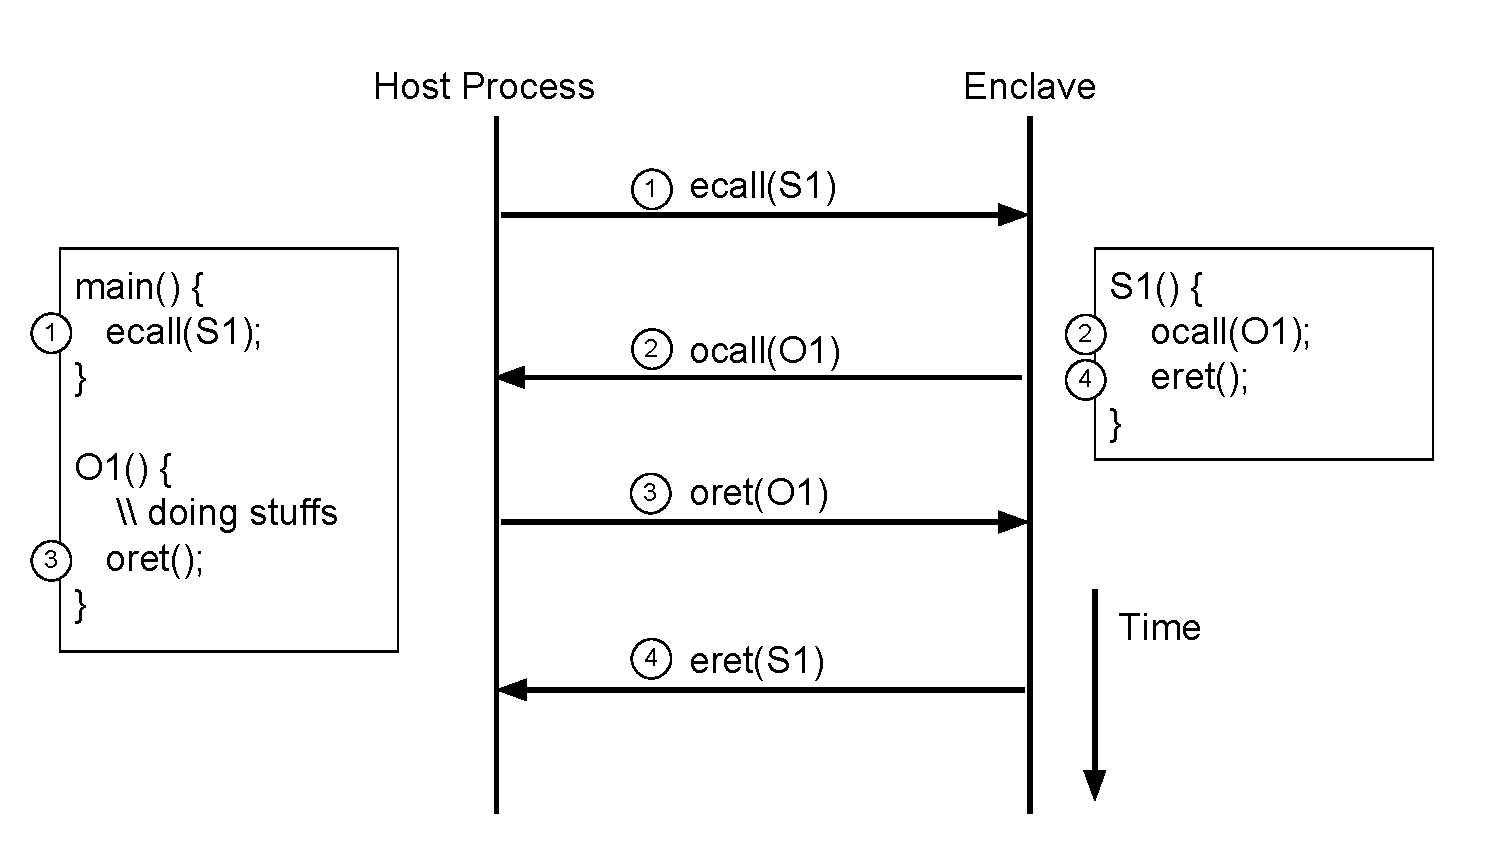
\includegraphics[width=0.7\textwidth]{fig_c5/synch-exit.pdf}
	\caption[SGX-Host interaction.]{Example of interaction between host 
		process and enclave by using the Intel SGX SDK. The host process 
		invokes 
		the secure function S1 from the main function (\texttt{ECALL}). S1 
		function 
		invokes O1 (\texttt{OCALL}), and this latter returns to S1 
		(\texttt{ORET}). 
		Finally, S1 returns back to the main function (\texttt{ERET}).}
	\label{fig:synch-exit}
\end{figure}

\subsection{OCALL Context Setting}
\label{ssec:ocall-context}

The \texttt{ocall\_context} is the structure that holds the enclave state once 
an \texttt{OCALL} is invoked.
The way in which the structure is set slightly differs between Intel SGX SDK 
before and after version $2.0$.
In this discussion, we consider the case of the Intel SGX SDK greater than 
$2.0$. However, a similar approach can be also applied to previous versions.

%When the execution leaves the enclave due to an \texttt{OCALL}, the 
%\texttt{tRts} creates a new \texttt{ocall\_context} structure on the stack as 
%described in Figure~\ref{fig:sgx-ocall-context}.
New \texttt{ocall\_context}es are located on top of the stack, as shown in
Figure~\ref{fig:sgx-ocall-context}, moreover, the new structures should 
follow a specific setting.
% shows the \texttt{ocall\_context} structure 
%and how it is allocated in the stack space.
In particular, three \texttt{ocall\_context} fields should be tuned: 
%\texttt{pre\_last\_sp}, \texttt{ocall\_ret}, and  \texttt{rbp}.
\begin{itemize}
	\item \texttt{pre\_last\_sp} must point to a previous 
	\texttt{ocall\_context} or to the stack base address. 
	This needs to handle a chain of nested \texttt{ECALL}s, which are basically 
	\texttt{ECALL}s performed by an outside function.
	\item \texttt{ocall\_ret} is used from SDK $2.0$ to save extended process 
	state~\cite{intel-xsave}. 
	More precisely, the system allocates a \texttt{xsave\_buff} pointed by 
	\texttt{ocall\_ret}. This buffer must be located after the new 
	\texttt{ocall\_context}.
	\item \texttt{rbp} must point to a memory location that contains the new 
	frame pointer and the return address, consecutively. This is because 
	the \texttt{asm\_oret()} function will use this structure as 
	epilogue~\cite{biondo2018guard}.
\end{itemize}
%It is important to underline that SGX does not use any security mechanism to 
%validate \texttt{ocall\_context} integrity.
It is important to underline that SGX does not validate \texttt{ocall\_context} 
integrity.
Therefore, an attacker that takes control of an enclave may craft a fake 
\texttt{ocall\_context}.
This problem has been existing in all SDK version available so far.
In the next section, we discuss why this is an underestimated problem 
and what threats can lead to.

\begin{figure}[t]
	\centering
	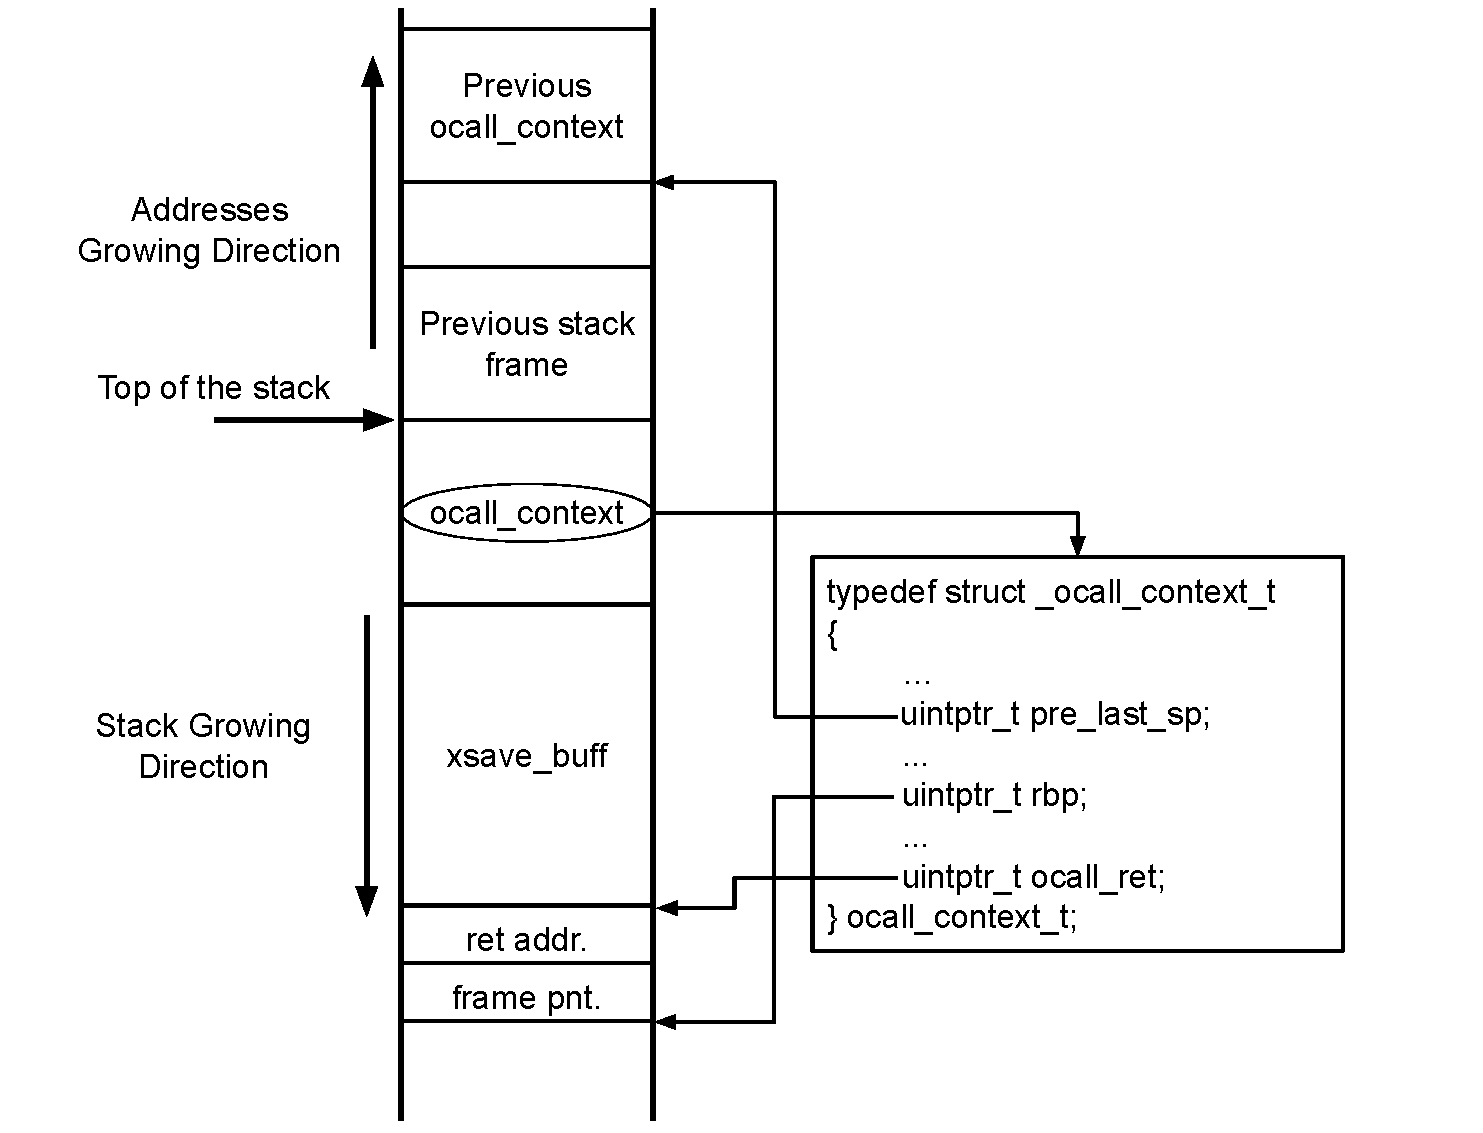
\includegraphics[width=0.75\textwidth]{fig_c5/sgx-ocall-context.pdf}
	\caption[\texttt{ocall\_context} memory layout.]{Example of 
	\texttt{ocall\_context} disposition in an enclave stack, the fields point 
	to structures within the stack itself in a precise order.}
	\label{fig:sgx-ocall-context}
\end{figure}

\subsection{Exploiting an ORET as a Trigger}
\label{ssec:oret-trigger}

%\todo{change the argumentation, bring at the beginning the issue and then 
%explain why through the dooret pseudo-code. So, finalize with the new threat.
%Otherwise it loos like a simple exposition of this problem.}
\texttt{ORET} is the only secure function that can trigger arbitrary code in an 
enclave. 
Therefore, an adversary enabled to abusing this function has also
privileged access to the enclave itself.
To understand why it is possible, we analyze the pseudo-code in 
Figure~\ref{fig:do_ocall}, which shows the \texttt{do\_oret()} secure function 
implementation.
%In \texttt{tRts}, \texttt{ORET} is implemented by the function 
%\texttt{do\_oret()}, whose a simplified pseudo-code is shown in 
%Figure~\ref{fig:do_ocall}.
Essentially, \texttt{do\_oret()} extracts the thread-local storage (TLS) from 
the current thread (Line~\ref{fig:do_ocall-getocont}).
The TLS contains information of the last \texttt{ocall\_context} saved.
After some formal controls (Line~\ref{fig:do_ocall-requirement}), the 
\texttt{ocall\_context} structure is used to restore the secure function 
execution through the \texttt{asm\_oret()} function 
(Line~\ref{fig:do_ocall-asmoret}).
%At first, \texttt{do\_oret()} extracts the TLS structure from the TCS 
%(Line~\ref{fig:do_ocall-gettls}).
%Then, it obtains the pointer to the last \texttt{ocall\_context} form the TLS 
%(Line~\ref{fig:do_ocall-getocont}).
%After this, \texttt{do\_oret()} performs a set of formal checks on 
%\texttt{ocall\_context} about its location 
%(Line~\ref{fig:do_ocall-requirement}).
%In case the formal checks are satisfied, \texttt{do\_oret()} sets TLS 
%\texttt{last\_sp} to the previous \texttt{ocall\_context} 
%(Line~\ref{fig:do_ocall-restocont}) and it invokes \texttt{asm\_oret()} to 
%restore \texttt{ocall\_context} (Line~\ref{fig:do_ocall-asmoret}).
%\texttt{asm\_oret()} is the function that actually sets processor state 
%according to \texttt{ocall\_context} values. Finally, \texttt{asm\_oret()} 
%resumes the secure function execution.
%Notice that \texttt{asm\_oret()} does not return, but it just passes the 
%control according to the \texttt{ocall\_context} setting.
%Therefore, if \texttt{do\_oret()} returns for any reasons, it is notified as 
%an error.
The formal checks performed by \texttt{do\_oret()} over the previous 
\texttt{ocall\_context} are quite naive.
There are three basic requirements:
\begin{enumerate*}[label=(\roman*)]
	\item the \texttt{ocall\_context} must be within the current stack space,
	\item the \texttt{ocall\_context} must contain a constant (hard-coded) 
	magic number, and
	\item the \texttt{pre\_last\_sp} must point before the actual 
	\texttt{ocall\_context}.
\end{enumerate*}

After the previous analysis, we realized that the Intel SGX SDK has no strict
mechanisms to verify the integrity of an \texttt{ocall\_context}.
In other words, any \texttt{ocall\_context} that fulfills
the previous conditions can be used to restore any context in an enclave.
First steps in this direction were explored by previous 
works~\cite{biondo2018guard}, which exploited \texttt{asm\_oret()} simply to 
control the processor registers in a one-shot code-reuse attack.
However, we want to push further the limitation of the Intel SGX SDK and show 
which consequences these issues can lead to.
%However, having a lack of \texttt{ocall\_context} checks can lead to 
%more serious consequences.
In fact, SnakeGX uses a combination of \texttt{ORET} and tampered 
\texttt{ocall\_context}es to restore arbitrary \emph{chains}
inside the enclave without performing further exploits.
In particular, SnakeGX abuses of this flaw for two reasons:
\begin{enumerate*}[label=(\roman*)]
	\item as a trigger to activate a custom payload hidden inside the 
	enclave;
	\item for the payload to perform a reliable context-switch between host and 
	enclave.
\end{enumerate*}
Therefore, crafting malicious \texttt{ocall\_context}es leads to the 
possibility of implanting backdoor in a trusted enclave without tampering the 
enclave code itself.
As such, the backdoor is shielded by the SGX features by design.
Moreover, the fact of using a single \texttt{ORET} to trigger the backdoor 
reduces the interactions required by a weak adversary for new attacks.
We discuss technical details in Section~\ref{sec:enclavekit} and show our 
proof-of-concept (PoC) in Section~\ref{sec:evaluation_snakegx}.

\begin{figure}[t]	
	\begin{lstlisting}[style=CStyle,escapechar=@]
	sgx_status_t do_oret()
	{
	// TLS structure
	tls = get_thread_data();@\label{fig:do_ocall-gettls}@
	// last ocall_context structure
	ocall_context = tls->last_sp;@\label{fig:do_ocall-getocont}@
	
	if (!formal_requirements(ocall_context))@\label{fig:do_ocall-requirement}@
	return SGX_ERROR_UNEXPECTED;
	
	// set TLS to point to previous ocall_context
	tls->last_sp = ocall_context->pre_last_sp;@\label{fig:do_ocall-restocont}@
	
	// restore last ocall_context
	asm_oret(ocall_context);@\label{fig:do_ocall-asmoret}@
	
	// in the normal execution
	// the control should not reach this point
	return SGX_ERROR_UNEXPECTED;
	}
	\end{lstlisting}
	\caption{Simplified \texttt{do\_oret()} pseudo-code.}
	\label{fig:do_ocall}
\end{figure}

\subsection{Mitigations}
\label{ssec:ocall-limitation}
%\todo{boh, not super sure of this stuff here}
There are many strategies to improve the \texttt{ocall\_context} integrity. 
A pure software solution could be computing an encrypted hash of 
\texttt{ocall\_context} when it is generated.
The hash might be appended as an extra field to the structure.
Another approach, instead, could be encrypting the entire structure itself.
However, pure software mitigation can be potentially bypassed by any 
code-reuse attack.
Once the attacker gains control of the enclave, she can basically revert or 
fake any encrypted processes.
A stronger solution could be introducing dedicated leaf functions that manage 
the generation and consumption of \texttt{ocall\_context}es.
For instance, during an \texttt{OCALL}, the enclave might use a dedicated leaf 
function that creates an \texttt{ocall\_context} and saves a 
copy (\ie an hash) in a memory location out of the attacker control (similar to 
TCS or SECS pages~\cite{costan2016intel}).
An \texttt{ORET}, then, should use another leaf function that performs extra 
checks and validate the integrity of the \texttt{ocall\_context}.
This solution might raise the bar for attacks, but it has two important 
drawbacks:
\begin{enumerate*}[label=(\roman*)]
	\item it forces Intel to re-thinking the SGX structures at low level,
	\item it leaves less freedom to developers that want to adapt the Intel SGX 
	SDK to their own needs (\eg to customize or introduce new structures).
\end{enumerate*}
After this consideration, we believe this issue would last for long before being
fixed. We reported this limitation to Intel that is reviewing its 
memory corruption protections.

\section{S\lowercase{nake}GX}
\label{sec:enclavekit}

%\todo{new messages to pass: (1) the framework has to achieve: persistence, 
%state, interactiveness; (2) the new challenges of implanting and designing the 
%framework.}

SnakeGX is the first framework that facilitates the implanting of persistent, 
stateful, and interactive backdoors inside SGX enclaves.
%This allows an adversary to inject additional secure functions without breaking
%the victim enclave functionality.
The framework design is challenging because we want to preserve the original
enclave functionality and configuration.
Even though SGX $2.0$ encompasses run-time page permissions 
setting~\cite{intel-sgx2}, an unexpected configuration may attract analysts 
attention (\ie the host can read the enclave page permissions).
On the contrary, our solutions purely rely on code-reuse techniques that do not
affect the enclave functionality and configuration.
%We achieve our goal despite the strict SGX threat model.
To the best of our knowledge, no previous works on SGX code-reuse attacks
never addressed these challenges.
We also recall we assume two conditions:
\begin{enumerate*}[label=(\roman*)]
	\item the target enclave has to be built with the Intel SGX SDK, 
	and
	\item it contains at least one exploitable memory-corruption 
	vulnerability (\eg a stack-based buffer overflow).
\end{enumerate*}

%In this paper, we propose SnakeGX: a framework to implant data-only 
%backdoors in SGX enclaves. 
%The strict threat model of this technology complicates 
%all the phases of a successful infection. To the best of our knowledge, all 
%these challenges 
%have never been discussed and addressed by previous works on SGX code-reuse 
%attacks.
%In this section, we illustrate all the challenges that we faced
%and discuss the solutions adopted when we designed our framework.
%In addition, we recall that we assume two conditions.
%First, the target enclaves have to be built with the SGX SDK.
%Second, the application running inside the enclave has at least one code 
%execution vulnerability that an attacker 
%can exploit (\eg a stack-based buffer overflow in a secure function).


\subsection{Overview}
\label{ssec:overview-attack}

%Our aim is to implant a backdoor inside a trusted thread of a trusted enclave.
The backdoor implanting is composed by three main phases:
\begin{enumerate*}[label=(\roman*)]
	\item enclave memory analysis,
	\item installation phase, and
	\item payload triggering.
\end{enumerate*}

\textbf{Enclave Memory Analysis.}
In this phase, the attacker has to achieve two goals:
\begin{enumerate*}[label=(\roman*)]
	\item inspect the process memory layout to identify enclave elements, and
	\item find a suitable location to install SnakeGX.
\end{enumerate*}
Since SGX does not implement any memory layout randomization, an adversary
can easily inspect the victim process memory by only using user-space 
privileges (\eg the enclave pages are assigned to a virtual device called 
\emph{isgx} in Linux environments).
Moreover, we target enclaves made with the Intel SGX SDK that follow the 
Enclave Linear Address Range (ELRANGE)~\cite{costan2016intel}.
As a result, an adversary with solely user-space privileges can obtain:
\begin{enumerate*}[label=(\roman*)]
	\item the enclave base address,
	\item the size, and
	\item the enclave trusted thread locations.
\end{enumerate*}
In Section~\ref{ssec:memory-location}, we discuss how to obtain a reliable 
memory location.

%\paragraph{Payload Installation.}
\textbf{Payload Installation.}
The installation phase is a one-shot attack that exploits an enclave 
vulnerability and uses a code-reuse technique for installing the payload.
This attack has to achieve three goals:
\begin{enumerate*}[label=(\roman*)]
	\item copy the payload inside an enclave (\eg the \emph{chain} and the 
	fake \texttt{ocall\_context}),
	\item set a hook to trigger the payload,
	\item resume the normal application behavior.
\end{enumerate*}
These three goals make this phase quite critical for three reasons. 
First, either enclave and host process have to remain available after the 
payload installation, or else we have to re-start the enclave.
Second, the enclave behavior does have not to change, or else the host should 
realize the attack.
%This means that the enclave secure functions have to work normally after the 
%payload installation.
Finally, we have to remove the payload in the untrusted memory, or else it 
could be detected.
This phase can be implemented by using any current code-reuse attacks for SGX
enclaves~\cite{lee2017hacking,biondo2018guard}.

\textbf{Payload Triggering.}
After the installation phase, the adversary only needs to trigger an
\texttt{ORET} to activate the payload 
(Section~\ref{ssec:set-a-payload-trigger}).
This allows an external adversary to activate the payload without attacking
the enclave from scratch.
%In this way, it is possible to trigger the payload transparently.
%Specifically, the hook will trigger the payload whenever the host application 
%interacts with the infected enclave. 
The payload contains the logic for interacting with the OS and the 
enclave.
To achieve persistence, we design a generic architecture that fits the SGX
realm (Section~\ref{ssec:enclave-kit-architecture}).
Moreover, since the payload can potentially leave the  
enclave, we designed a generic context-switch mechanism that
enables the payload to keep control over the enclave 
(Section~\ref{ssec:switch-context}).

\subsection{Getting a Secure Memory Location}
\label{ssec:memory-location}

%\todo{start the argumentation by saying: due to our analysis, we think using a 
%trusted thread is the best option because: 1) sgx error design, 2) we can't 
%allocate new pages.}
%Due to the strict SGX security features, 
We employ a trusted
thread as backdoor location because it allows us to abuse the 
design error described in Section~\ref{sec:sgx-internal}.
%	\item SGX does not allow to arbitrarily allocate memory 
%	pages.\footnote{The new SGX SDK versions can add only a predefined 
%	number of pages~\cite{intel-sgx2}.}
%\end{enumerate*}
%Therefore, obtaining a suitable memory location for an SGX data-only 
%malware is challenging.
If an enclave does not have any available trusted thread, 
SnakeGX can still work by stealing one of the available threads. In this 
case, the target application may notice some degradation of the performances. 
However, the system does not raise any exception because it is not possible to 
determinate the real cause.
In this way, we can take control of an enclave trusted thread without affecting 
enclave functionality.
%As we describe in Section~\ref{ssec:thread-handling}, SGX SDK uses a bind 
%mechanism that is implemented in the \texttt{uRts} libraries.
%This maintains a pool of trusted thread that is bounded to an untrusted one 
%on-demand.
%For instance, in a Linux environment the trusted threads are stored in a 
%\texttt{std::vector}.
%In addition, controlling a trusted thread allows us to abuse of SDK error 
%designs discussed in Section~\ref{sec:sgx-internal}.
These properties are SGX specific and were not considered in previous 
code-reuse works.

\paragraph{\textbf{Un-releasing a Trusted Thread.}}
This technique is based on a misbehaviour of the thread binding mechanisms in 
the \texttt{uRts} library.
Once a secure function is invoked through the Intel SGX SDK, the
\texttt{uRts} searches a free trusted thread and marks it as \emph{busy}.
Then, the trusted thread is released when the secure function ends.
However, an attacker can exploit a secure function and leaves the enclave 
skipping the \emph{releasing} phase in the \texttt{uRts}.
As a result, the trusted thread remains \emph{busy} and it will never
be assigned to future executions, in this way it is stolen.
The strategy of this technique is composed by two phases:
\begin{enumerate*}[label=(\roman*)]
	\item invoking and exploiting a secure function, then
	\item exiting from the enclave (\eg by using EEXIT) and 
	skipping the \emph{releasing} of the trusted thread.
\end{enumerate*}
This approach requires the enclave has at least two trusted threads, otherwise 
the application might realize that the enclave is unavailable.
We use this approach for our PoC.

\paragraph{\textbf{Making a New Thread.}}
SGX $2.0$ and recent versions of the Intel SGX SDK allow creating trusted 
threads at run-time.
Therefore, an attacker may force the enclave to create a new trusted thread 
without tampering with the pool.
However, this approach should be used wisely, otherwise unexpected trusted 
threads may attract the analyst attention, thus affecting the stealthiness of 
SnakeGX.

\subsection{Set a Payload Trigger}
\label{ssec:set-a-payload-trigger}
We design our trigger on top of the Intel SGX SDK flaw highlighted in 
Section~\ref{sec:sgx-internal}.
We assume that an attacker has already gained control of an enclave by means
of a code-reuse attack.
Moreover, either the payload and the trigger must be tuned for the trusted 
thread under attack.

To install the trigger, the adversary has to mimic an \texttt{OCALL}
such that 
the next \texttt{ORET} will activate the backdoor (\ie a \emph{chain}) instead 
of resuming the execution of a secure function.
To achieve this goal, the adversary has to perform three main operations:
\begin{enumerate*}[label=(\roman*)]
	\item set a fake \texttt{ocall\_context} on the stack that satisfies the 
	formal requirements as described in Section~\ref{ssec:ocall-context};
	\item call the function \texttt{save\_xregs()} (which is contained in 
	\texttt{tRts}) to save extended process features, the function should take 
	as an argument the \texttt{xsave\_buff} location of the fake 
	\texttt{ocall\_context} previously copied;
	\item call the function \texttt{update\_ocall\_lastsp()} (which is 
	contained in \texttt{tRts}) by passing the pointer to the fake 
	\texttt{ocall\_context}. This function will set TLS \texttt{last\_sp} 
	to the fake \texttt{ocall\_context}, thus simulating an \texttt{OCALL}.
\end{enumerate*}

This setting allows us to resume the payload execution by performing an 
\texttt{ORET} on the attacked trusted thread.
More precisely, \texttt{asm\_oret()} will restore the context previously 
installed and it will activate the first gadget.
By default, \texttt{ocall\_context} does not perform a pivot (\ie it does not 
set the \texttt{rsp} register).
To bypass this issue, we used a pivot gadget that is contained in 
\texttt{asm\_oret()} function itself:\textsl{} \texttt{mov rsp, rbp; pop rbp; 
	ret}.
This gadget is present in any SDK version released so far, so it is a generic 
technique for SGX backdoors.
We observed the same gadget also in Windows \texttt{tRts}.
%That is, the return address in the fake \texttt{ocall\_context} points to a 
%pivot gadget. % ERI UBRIACO?
%Therefore, the return address in the fake \texttt{ocall\_context} points to 
%a pivot gadget. 
Therefore, the first instruction triggered by the fake \texttt{ocall\_context} 
is a pivot gadget.
Then, we set the \texttt{rbp} to point to a fake stack inside the stolen 
thread. 
In this way, the \texttt{ORET} always pivots to the fake stack that contains 
the actual payload.
%When a process invokes an \texttt{ORET} on the compromised TCS, the 
%\texttt{do\_oret} function will restore the fake \texttt{ocall\_context}.
%As a result, the \texttt{tRts} will trigger our payload instead of resuming a 
%secure function.
Notice that this mechanism just pivots to the fake address indicated by the 
fake \texttt{ocall\_context} (\ie \texttt{rbp}).
As such, an attacker only needs one fake \texttt{ocall\_context} that pivots to 
a fixed location.
Then, she can just copy different fake stacks to the same location to activate 
different payloads.


\subsection{Backdoor Architecture}
\label{ssec:enclave-kit-architecture}

Figure~\ref{fig:t-thread-stack-installed} shows the payload
architecture that we adopted for SnakeGX.
This solution allows us to achieve payload persistence in an SGX enclave by 
only using the stack address space.
By default, the Intel SGX SDK sets the stack size at $40$KB, therefore, we 
design SnakeGX to fit this size.
For the sake of simplicity, we describe the switching mechanism in 
Section~\ref{ssec:switch-context}.

As underlined in~\cite{vogl2014persistent}, classic code-reuse attacks (\eg 
ROP) are designed to be one-shot.
After executing a \emph{chain}, it may be destroyed due to gadgets side effects.
Therefore, we need a location to keep a backup of the structures used.
According to this consideration, we split the stack address memory in four 
sections:

\textbf{Fake Frame.} SnakeGX requires a dedicated location for installing 
an \texttt{ocall\_context}.
This structure is used to either perform the payload trigger and the 
context-switch (see Section~\ref{sec:sgx-internal}).
These features are crucial to implement a persistent backdoor in the SGX 
realm since classic techniques cannot be used.

\textbf{Buffer.} This area contains temporary variables that are used by  
payloads. For instance, our PoC stores the previous data 
exfiltrated (see Section~\ref{sec:evaluation_snakegx}).

\textbf{Workspace.} The fake frame previously installed is tuned to pivot the 
execution to this location. 
Generally speaking, any payload is coped here before being executed.

\textbf{Backup.} This location contains a copy of all the structures 
needed by SnakeGX to work properly.
After the SnakeGX installation, this location should not be overwritten.
%\end{itemize}

%Since a data-only malware must be designed to re-install itself after being 
%triggered.
Since the \emph{chains} used may be destroyed after 
payload execution, we need a mechanism that brings SnakeGX to the initial 
state after the payload has been executed.
More precisely, it has to make the payload available for future invocations.
To achieve this goal, we use three \emph{chains}: Boot Chain (B$_c$), Payload 
Chain (P$_c$), and Reset Chain (R$_c$).
Each of them is formed by a fake stack that is maintained in the backup zone 
and moved in the workspace on demand:

\textbf{Boot Chain (B$_c$).} This is the first chain that is triggered by 
the hook, its duties are:
\begin{enumerate*}[label=(\roman*)]
	\item copy P$_c$ and R$_c$ into the workspace, and
	\item pivot to P$_c$.
\end{enumerate*} 
This chain is usually quite short.

\textbf{Payload Chain (P$_c$).} This contains the actual payload 
and is strictly enclave dependent. When the payload ends, it just pivots to 
R$_c$.

\textbf{Reset Chain (R$_c$).} 
This \emph{chain} resets the payload inside the enclave and makes it ready for 
the next calls without the need of the installation phase.
This is achieved with the following operations:
\begin{enumerate*}[label=(\roman*)]
	\item copy B$_c$ into workspace,
	\item copy the \texttt{ocall\_context} in the fake frame,
	\item set TLS to point to \texttt{ocall\_context}.
\end{enumerate*}

After the execution of R$_c$, SnakeGX can be triggered again by a new 
\texttt{ORET}.
The loop boot-payload-reset \emph{chain}, along the architecture shown in 
Figure~\ref{fig:t-thread-stack-installed}, is a simple framework that can be 
used by the adversaries to design their customized payload for SnakeGX.

\begin{figure}[t]
	\centering
	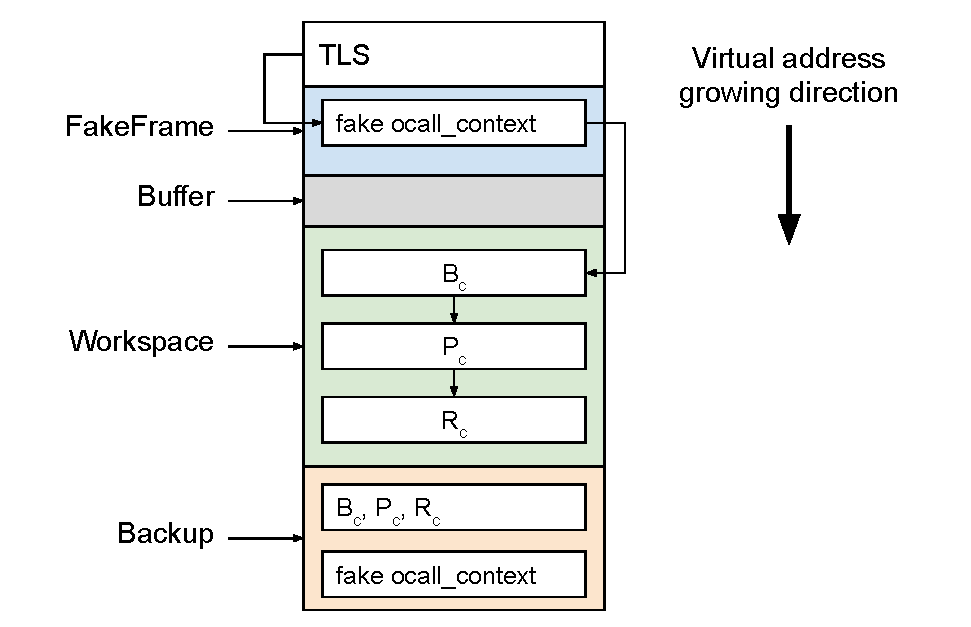
\includegraphics[width=0.6\textwidth]{fig_c5/t-thread-stack-installed.pdf}
	\caption[SnakeGX installation layour.]{Trusted thread stack after SnakeGX 
	installation. The memory is split in four areas: FakeFrame, buffer, 
	workspace, and backup. Moreover, the stack contains copies of B$_{c}$, 
	P$_{c}$, and R$_{c}$.}
	\label{fig:t-thread-stack-installed}
\end{figure}

\subsection{Context-Switch}
\label{ssec:switch-context}

To allow SnakeGX to interact with the host OS, while 
maintaining the enclave control,
%we need novel methods never used for previous any data-only malware.
%SnakeGX is able to interact with the
%host OS while maintaining the enclave control.
%To achieve this goal, 
%Overall, 
we need to perform three operations:
\begin{enumerate*}[label=(S\arabic*)]
	\item temporarily copy part of the payload outside,
	%\item exit gracefully, and
	\item leave the enclave, and
	\item resume the execution inside the enclave.
\end{enumerate*}
The first two operations are relatively simple: the Intel SGX SDK already 
provides standard routines (\eg \texttt{memcpy})
to move data outside the enclave.
Moreover, it is possible to pivoting outside the enclave by abusing the 
\texttt{EEXIT} opcode (Section~\ref{sec:background}). 
On the contrary, resuming the enclave execution requires SnakeGX to invoke
an \texttt{EENTER} opcode.
However, it is not possible to arbitrarily jump inside an enclave (\ie the 
entry point is fixed).
Therefore, we abuse again of the Intel SGX SDK deign error described in 
Section~\ref{sec:sgx-internal}.

To perform the context-switch, we split the payload in three chains, called 
outside-chain 
(O$_c$), payload-one (P$_1$), and payload-two (P$_2$).
O$_c$ is the part of the payload copied in the untrusted memory,
while P$_1$ and P$_2$ remain inside the enclave.
During the context-switch, we execute P$_1$, O$_c$, and P$_2$, 
consequently.
More precisely, once P$_1$ requires to interact with the host, it performs (S1) 
to prepare the O$_c$ activation, installs a fake frame
(Section~\ref{ssec:enclave-kit-architecture}), and prepares P$_2$ in the 
workspace.
At this point, P$_1$ can perform (S2): leave the enclave and pivot to 
O$_c$.
When the operations in untrusted memory are terminated, O$_c$ only needs to run 
an \texttt{ORET} that will activate P$_2$ (S3).
Finally, P$_2$ can clean the traces left by O$_c$ and continue the backdoor 
execution.
It is possible to perform many context-switch by tuning the payload accordingly.

\section{Evaluation}
\label{sec:evaluation_snakegx}

We evaluate the real impact of our framework against StealthDB~\cite{stealthdb},
an open-source project that leverages on the SGX technology.
We opted for StealthDB because it is a generic representation of our scenario, 
as we describe in Section~\ref{ssec:stealthdb}.
We split our evaluation in three parts:
\begin{enumerate*}[label=(\roman*)]
	\item a technical discussion of our use-case 
	(Section~\ref{ssec:homemade-poc}),
	\item a measurement of the traces left (Section~\ref{ssec:comparison}), and
	\item a discussion about the countermeasures (Section~\ref{ssec:detection}).
\end{enumerate*}

\subsection{StealthDB}
\label{ssec:stealthdb}
StealthDB~\cite{stealthdb} is a plugin for PostgreSQL~\cite{postgresql} that
uses Intel SGX enclaves to implement an encrypted database.
This project is the ideal use-case for SnakeGX: StealthDB lifetime is bounded 
to PostgreSQL, thus we can rely on its enclaves as a secure save point for 
storing the payload and launching the attacks.

StealthDB uses a single SGX enclave to handle encrypted fields and operations 
that are performed inside the enclave itself.
In this way, the database can securely save encrypted fields on disk, while the
plain values are handled only inside the enclave.
The encryption algorithm is AES-CTR with keys 128 bits long. These keys are 
sealed on 
the disk through the standard SGX features.
A user can define multiple keys that are loaded on-demand inside 
the enclave, however, the StealthDB enclave maintains in memory only a single 
key at a time.
In this scenario, one-shot state-of-the-art techniques 
require multiple interactions to obtain all the keys. 
This approach leaves more copies of the payload in the memory, thus increasing
the risk of being detected.
Even if an adversary manages to obtain all the sealed keys, she still has 
to perform new attacks whenever a new key is generated.
SnakeGX is able to understand when a new key is loaded and performs the 
exfiltration steps accordingly. In this way, the attacker transparently hides 
and activates complex logic that resides inside a trusted enclave. 

\subsection{Use-Case Discussion}
\label{ssec:homemade-poc}

In this section, we discuss the properties of 
our PoC payload and some implementation details. For more technical 
details about our payload see Appendix~\ref{ssec:my-rop-chain}.
Our setup is composed by an application that loads StealthDB enclave 
and performs the attacks.
We extracted the gadgets for the \emph{chains} by running
ROPGadget~\cite{ropgadget} on the compiled enclave.
As our threat model details in 
Section~\ref{sec:threat-model_snakegx}, we introduced a memory corruption 
vulnerability 
in StealthDB to simplify the payload delivery.
We developed our data-only malware for SGX in a host OS running Linux with 
kernel $4.15.0$ and Intel SGX SDK version $2.9$.

We composed our PoC of three steps.
First, the application starts and loads the enclave.
Second, we exploit the enclave vulnerability and implant 
the payload.
Third, we alternatively invoke normal secure functions and
the backdoor. This shows that SnakeGX does not alter the normal enclave 
functionality.
Once the backdoor is triggered, SnakeGX exfiltrates the keys only when the 
condition is satisfied.
Without using SnakeGX, the adversary has to perform many 
attacks to achieve the same goal, which potentially leaves traces for an 
analyst.
Moreover, SnakeGX avoids the burden of crafting new payloads at each 
exfiltration.

\textbf{The Payload.}
Our payload shows three important features:
\begin{enumerate*}[label=(\roman*)]
	\item persistence,
	\item internal state, and
	\item context-switch.
\end{enumerate*}
More precisely, the payload exfiltrates a key if and only if it changes.
This is crucial in our threat model (Section~\ref{sec:threat-model_snakegx}), 
which 
assumes a non-compromised host, thus the attacker has to reduce 
un-useful actions.
In fact, all the payload structures are kept inside the enclave,
and an adversary only needs to trigger an \texttt{ORET} against the compromised
thread.
Once activated, the payload is able to self-check its status, and in case, leak 
the key.
The payload is composed by three \emph{chains}:
\begin{itemize}
	\item \textbf{P$_1$} is the first payload to be activated. It checks if the 
	key changed, and in case activates the exfiltration.
	\item \textbf{O} is the outside-chain that actually exfiltrates the key. 
	It 
	is temporary copied in the untrusted memory by P$_1$.
	\item \textbf{P$_2$} is the second payload that is triggered by O after 
	the 
	exfiltration. The purpose of P$_2$ is to wipe out all the temporary 
	structures 
	previously copied in the untrusted memory, \ie O and the key.
\end{itemize}
From an external analyzer, all the structures (\ie P$_1$, P$_2$, and O) are 
always
contained in the enclave when the payload is not activated.
The only \emph{chain} temporary copied outside is O, but P$_2$ cleans its 
traces.
Moreover, to activate the payload, the attacker only needs to trigger an 
\texttt{ORET} 
instead of preparing complex code-reuse attacks.
In Section~\ref{ssec:comparison}, we measure and compare the traces of SnakeGX
\wrt the state-of-the-art attacks.

\textbf{Chains Composition.}
\label{ssec:chain-composition}
Our payload maintains an internal state and interacts with the 
host.
To handle the state, the payload is able to perform a conditional pivoting
by comparing the current key and a copy of the last key 
exfiltrated~\cite{geometry2007}.
The conditional chain is implemented in P$_1$.
Once the key changes, P$_1$ will pivot to a \emph{chain} that performs the 
exfiltration. Otherwise, the payload will pivot to 
another \emph{chain} that simply resumes the normal enclave behavior.
We describe the gadgets used to perform conditional pivoting in 
Appendix~\ref{app:condition-gadget}.
The interaction with the OS, instead, requires two types of \emph{chains}: some 
that run inside the enclave (\ie P$_1$ and P$_2$), and others that run outside
(\ie O).
Table~\ref{tbl:gadgets} shows some statistics about \emph{chains} composition.
The \emph{chains} inside the enclave are entirely composed by gadgets from the 
\texttt{tRts}.
More precisely, P$_1$ and P$_2$ invokes $27$ and $13$ functions such as 
\texttt{memcpy()}, and \texttt{update\_ocall\_lastsp()}, respectively.
In terms of memory, P$_1$ and P$_2$ occupy $2816$ and $1232$ byes, 
respectively.
The chain O, instead, is composed by classic gadgets from \texttt{libc}.
More precisely, O is composed by $20$ small standard gadgets. 
The internal ecosystem of \texttt{tRts}, and the \texttt{libc} in Linux 
systems, provide
enough gadgets and functions to create useful payloads.
We describe the gadgets used for these \emph{chains} in 
Appendix~\ref{app:context-switch-chain}.

\begin{table}[t]
	\centering
	%	\vspace{-7.5em}%
	\begin{tabular}{lrrr}
		\toprule
		Chain & \multicolumn{1}{l}{\# fnc/sys} & \multicolumn{1}{l}{\# gadgets} 
		& \multicolumn{1}{l}{size [B]} 
		\\ \midrule
		P$_1$    & $27$ & $23$ & $2816$ \\
		P$_2$    & $13$ &  $7$ & $1232$ \\
		O     	 & $4$ &  $20$ & $312$ \\ \midrule
		sum   	 & $44$ &  $50$ & $4360$ \\ \bottomrule
	\end{tabular}
	\caption{Statistics of the gadgets used for the payload.}
	\label{tbl:gadgets}
\end{table}

\subsection{Trace Measurements}
\label{ssec:comparison}
We analyze our PoC and measure the advantages SnakeGX introduces.
We recall that our threat model assumes a weak adversary which has no control 
of the host, and therefore, she has to improve her stealthiness.
To perform the same goal of our PoC by using state-of-the-art one-shot 
attacks~\cite{biondo2018guard}, an attacker has to leave in the untrusted 
memory around $4$KB of structures (\ie P$_1$, P$_2$ and O).
These traces can be found by using previous results already shown in the 
literature~\cite{stancill2013check,polychronakis2011rop,kittel2015counteracting,Graziano:2016:RFA:2897845.2897894}.
Moreover, their identification results even simpler since
they use peculiar structures such as 
\texttt{sgx\_exception\_info\_t} (see Appendix~\ref{ssec:my-rop-chain}).
On the contrary, SnakeGX requires only one \texttt{ORET} to trigger the
payload.
In particular, our PoC implements an \texttt{ORET} by using only $4$ gadgets 
and leaving a negligible footprint of $56$ byes in memory. 
%, thus, reducing its traces over $99\%$.
As a result, the trigger used by SnakeGX is able to activate payloads 
arbitrary complex by leaving a minimal footprint.

\subsection{Countermeasures}
\label{ssec:detection}

SnakeGX poses new challenges for forensic investigators and backdoor analysts 
as well as for experienced reverse engineers.
The current state-of-the-art tools cannot detect and dissect this new threat. 
It is necessary to develop 
new tools and techniques for the detection and possibly the prevention of 
threats affecting SGX and similar technologies.
Here, we discuss some possible directions for the detection that can be used to 
observe the presence of SnakeGX in a system.
Moreover, we analyze how the current state-of-the-art defenses
can mitigate our attack and which future research lines can be taken.
This is not a comprehensive study and we leave this part for future work.
We hope this research paves the way for new works in the malware analysis field.

\textbf{Memory Forensic Analysis.}
SnakeGX is an infector of legitimate enclaves and is by definition 
stealthier.
This means that any form of memory forensics is no more possible. The memory of 
the enclave cannot be inspected. As explained in Section~\ref{sec:background},
SGX makes impossible to read memory pages that belong to an enclave.
Any attempts at reading such pages will result in a fake value $0$xFF.
Another possible approach is to use new attacks based on 
microcode flaws~\cite{foreshadow} or fault 
injections~\cite{Murdock2019plundervolt} to dump an enclave content.
Alternatively, it is possible to use side-channel attacks to 
infer specific enclave manipulations, as discussed in~\cite{216033}.
It should also be pointed out that it is still possible to retrieve 
\texttt{uRts} information.
For instance, we could compare the number of trusted threads in \texttt{uRts} 
and 
the number of trusted threads in the \texttt{ELRANGE} structure.
An inconsistency will bring to clues regarding the state of that enclave.

\textbf{Sandboxes.}
Recently, researchers proposed sandboxes to reduce the 
interaction of a malware-enclave and the system~\cite{sgxjail}.
These solutions are designed for systems that cannot assess the 
origin of an enclave beforehand, thus they do not trust it.
These defenses can, in principle, reduce the attack surface of SnakeGX.
However, since we target only systems that host known and trusted enclaves, we 
do not expect sandboxes in place.
In the worst case, we can still detect the presence of a sandbox by probing the 
process (\ie through a syscall) and interrupt the attack.

\textbf{Syscalls Trace.}
Even though the payload is hidden from reading,
it is still possible to analyze the syscall interaction of the outside-chains.
This approach has been extensively studied and it is quite common in the field 
of malware analysis.
%This is a typical approach for malware detection.
Researchers may design a tracer and superficially focus on the interaction with 
the enclave.
For instance, this tool may spot that SnakeGX generated a file operation that 
did not appear in previous interactions. In this way, analysts can infer the 
behaviour of the code inside the enclave.

\textbf{Control Flow Integrity Checks.}
Control Flow Integrity checks (CFI) are strong weapons already used
in standard programs to mitigate code-reuse attacks.
Such mechanisms rely on different strategies to force a program to execute only 
valid paths at run-time.
In the current enclave implementation, the system relies on
classic stack canary to avoid buffer overflow.
However, Lee et al.~\cite{lee2017hacking} discussed a technique to bypass such 
protection.
Other non-standard systems, such as SGX
Shield~\cite{seo2017sgx}, implement a custom CFI to mitigate these
issues.
However, Biondo et al.~\cite{biondo2018guard} managed to bypass
their protection too.
So far, there are not effective defenses against code-reuse attacks in the 
context of enclaves.
This approach might raise the bar for attackers who would attempt to deploy 
SnakeGX or to perform code-reuse attacks in general.

\textbf{Detecting Fake Structures.}
SnakeGX exploits the possibility to craft fake structures
that are used in critical \texttt{tRts} functions, \ie \texttt{ocall\_context}.
We deeply analyzed this issues and proposed mitigation strategies in 
Section~\ref{ssec:ocall-limitation}.

\section{Discussion}
\label{sec:discussion_snakegx}

Here, we discuss various aspects of SnakeGX generalization.

\subsection{SnakeGX Portability}
The current implementation of SnakeGX is based on a specific version 
of the Intel SGX SDK, for a specific application and operating system.
In this section, we study the portability of our PoC and show the approach 
is generic and can be easily adapted to other SDKs and OSs.
%We study the portability of SnakeGX in other scenarios.
%Recently, new TEE frameworks were proposed on the market, or as research 
Recently, new SGX frameworks were released on the market, or research 
prototypes, to provide an abstraction layer that simplifies the enclave 
development.
In particular, projects such as Open Enclave~\cite{openenclave}, Google 
Asylo~\cite{gasylo}, and SGX Shield~\cite{baumann2015shielding} 
use the standard Intel SGX SDK to perform host 
interaction (\ie \texttt{OCALL}/\texttt{ORET}), thus inheriting the same 
limitations described in Section~\ref{sec:sgx-internal}.
From our point of view, we can implant SnakeGX in any enclave developed with 
these frameworks if they follow our threat model assumptions 
(Section~\ref{sec:threat-model_snakegx}).
We also analyzed the Intel SGX SDK for Windows, in which we found and tested 
the same flaw described in our work.
Finally, the standard \texttt{tRts} libraries contain all the gadgets used in 
our PoC.
In general, SnakeGX can potentially affect enclaves developed on different
SDKs as long as: 
\begin{enumerate*}[label=(\roman*)]
	\item they are abstraction layers of the Intel SGX SDK, or
	\item they use a host interaction that relies on unprotected structures 
	like \texttt{ocall\_context}.
\end{enumerate*}
In this paper, we proposed an instance of SnakeGX targeting StealthDB on Linux. 
However, the idea is generic and the persistence, stateful, and context-switch 
properties can be found and achieved also in other OSs and popular SDKs based 
on the Intel one.

\subsection{Persistence Offline}
%\textbf{Persistence Offline.}
%\subsection{Persistence Offline}
%Similar to Vogl work~\cite{vogl2014persistent}, SnakeGX keeps persistence in 
%memory as long as the host enclave is loaded. 
SnakeGX maintains persistence in memory as long as the host enclave is loaded.
This is similar to what Vogl et al.~\cite{vogl2014persistent} have shown with 
``Chuck''.
In their proof of concept they achieved persistence on the running system. 
Their ROP rootkit did not survive after reboot.
%In our scenario, to achieve a full persistence once the enclave is restarted, 
%we should exploit sealing mechanism.
In our scenario, SnakeGX may achieve a more complete persistence by exploiting 
the sealing mechanism.
In this case, the malicious payload would not be affected if the enclave is 
restarted.
%That is, a common SGX practice is saving enclave statues (\ie its data) before 
%the enclave shouts down.
This sealing mechanism is a common SGX practice. It saves the enclave state 
(\ie its data) before the enclave shuts down.
%This is done by using a sealing mechanisms, if the victim enclave has a 
%loophole in the restoring phase, this could be exploited to inject SnakeGX 
%again after a reboot.
If the victim enclave has a loophole in the restoring phase, this could be 
exploited to inject SnakeGX again after a reboot.
However, this is strictly enclave-dependent and therefore we did not include in 
our discussion and it is left for the future.

%\todo{loose persistence once the enclave is switched off.}
\subsection{SnakeGX 32bit}
%\paragraph{SnakeGX 32bit.}
%\todo{32 bits.}
In this paper, we designed our PoC for $64$bit architectures.
%However, Intel allows $32$bit code to run in enclaves.
However, Intel SGX supports also $32$bit code to run in enclaves.
From our point of view, the main difference between $32$bit and $64$bit is the 
calling convention.
%Therefore, the techniques we used for SnakeGX can be adapted also in a $32$bit 
%scenario.
Therefore, the techniques we discussed and used for SnakeGX are still valid and 
can be easily
ported to $32$bit applications.
